
%%%%%%%%%%%%%%%%%%%%%%%%%%%%%%%%%%%%%%%%%%%%%%%%%%%%%%%%%%%%%%%%%%%%%%%%
\chapter{Probability and Statistics Analysis} \label{sec_probsnstat}
%%%%%%%%%%%%%%%%%%%%%%%%%%%%%%%%%%%%%%%%%%%%%%%%%%%%%%%%%%%%%%%%%%%%%%%%

%%%%%%%%%%%%%%%%%%%%%%%%%%%%%%%%%%%%%%%%%%%%%%%%%%%%%%%%%%%%%%%%%%%%%%%%
\section{Introduction to Probability and Statistical Analysis} \label{sec_statintro}
%%%%%%%%%%%%%%%%%%%%%%%%%%%%%%%%%%%%%%%%%%%%%%%%%%%%%%%%%%%%%%%%%%%%%%%% this may not be the best name?

% note to self: stats and probs discussion is very independt of sources/whys, think of this as presenting numbers only

As introduced in \autoref{env_info}, ambient noise in the Arctic can be partitioned into three environmental conditions: 'ice with duct', 'ice without duct', and 'no ice.' Each of these acoustic environments has a unique makeup of ambient noise produced by a variety of drivers and affected by the nature of the environment. By expanding the original frequency band, more information is gained of how ambient sound operates under each environment and the differences between them.  

 A broadband analysis of the ambient sound level (ANL) recorded by the SHRUS was performed using the data from SHRU5. To keep consistency with the original analysis \footcite[]{Bonnel2021}, the data for this analysis came from SHRU5, as it had the least self noise compared to other SHRUS. Each frequency band is 50 Hz wide and centered on frequencies from 50 to 1900, 50 Hz apart, for a total of 39 frequency bands. The range was chosen as the original sampling rate ($f_{s}$) of the SHRUs is  3906.2 Hz; by the Nyquist sampling frequency, the maximum reliable frequency that can be analysed is 1951.  These frequencies were divided into the three acoustic environments of 'ice with duct', 'ice without duct' and 'no ice'. % be sure to CLEARLY define these in section before

Though each frequency has some independent qualities, they appear to be quantitatively linked when analyzed using a myriad of different statistics. These statistic quantities ranged from single metrics to comparing probabilities of the entire acoustic environment. While the original paper examined a frequency band around 300 Hz of 250-350 Hz, it can be assumed that this was not the only frequency propagating through the water. As this analysis would suggest, the frequency range of ambient noise under ice is broad in nature, likely influenced by environmental drivers such as shifting ice \footcite[]{ice_enviro}. This discussion will primarily focus on the numerical quantities and probabilities of ambient sound collected during the duration of CANAPE, independent of time and sources.

% how refs cited kind open on mit website, this works


%%%%%%%%%%%%%%%%%%%%%%%%%%%%%%%%%%%%%%%%%%%%%%%%%%%%%%%%%%%%%%%%%%%%%%%%
\section{Probability and Statistical Analysis Methods and Results}
%%%%%%%%%%%%%%%%%%%%%%%%%%%%%%%%%%%%%%%%%%%%%%%%%%%%%%%%%%%%%%%%%%%%%%%%

%%%%%%%%%%%%%%%%%%%%%%%%%%%%%%%%%%%%%%%%%%%%%%%%%%%%%%%%%%%%%%%%%%%%%%%%
\subsection{Correlation Between Frequencies}
%%%%%%%%%%%%%%%%%%%%%%%%%%%%%%%%%%%%%%%%%%%%%%%%%%%%%%%%%%%%%%%%%%%%%%%%

Exploring the relationships between frequencies in probability shows these environmental conditions share a significant amount of distribution of ambient noise for many frequencies. One can infer that the ambient noise is broadband in nature as many of the previous figures show similar or same results through multiple bands of frequency. In \autoref{fig_freq_corr} the correlation between each of the ambient noise levels of each frequency is shown for each of the three environmental conditions. It is worth noting that the p-value for each of the correlations is an identity matrix, so the likely hood that the null hypothesis is true is zero percent; The exception is when the same frequency is compared against itself as the p-value is 1. The correlation values range from 0.4758 under the 'ice without duct' condition to 1 when frequencies are compared against themselves. 

Other than the very lowest frequencies, correlation between almost all of the frequency bands is quite high, lending credit to the idea that ambient noise encompasses many frequencies.  Each environmental condition does act differently when high and low frequencies are compared to each other, resulting in different shapes of the correlation graphs. The 'no ice' condition has distinct bands of correlation around 0.7 and 0.9 for the 100-200 Hz and 200-300 Hz comparisons; elsewhere is is approximately 1, resulting in a box-shaped block of high correlation values. 'No ice' has the largest area of high correlation values compared to 'ice without duct' and 'ice with duct'.

% not entirely sure if i am able to speculate as to why this is, this is just how it is
The 'ice without duct' condition has minima correlation along the edges of low frequency comparison. From the edges moving inwards, the correlation values increase to nearly 1. There appears to be more correlation between frequencies below 800 when compared to the 'no ice' condition graph, as the 'ice without duct' plot has a less boxy shape and a smoother gradient through correlation values. When high and low frequencies are compared, correlation values range from 0.7 to 0.8. 'Ice without duct' has the least amount of high correlation of \autoref{fig_freq_corr}, and is the least correlated of the three while still showing that many ANL frequencies are very related.

Correlation for the environmental condition 'ice with duct' has the same distinct bands of low correlation at low frequency as the other two graphs, but does not have as distinct of a green band corresponding to 0.7. 'Ice with duct' has a narrower band of high correlation than 'ice with duct' and the middle amount of high correlation values. From about 50 Hz to 1900 Hz correlation values are around 0.9, but once frequencies above 1000 are compared to frequencies below 1000 Hz, correlation drops to around 0.8. While \autoref{fig_freq_corr} definitively shows that many frequencies are closely related, the exact nature of their relationship is not yet shown. Metrics such as mean ANL and pairwise difference display more characteristics of the similarities and differences between the sound through this wide band of frequencies.

\begin{figure}[ht]
\centering
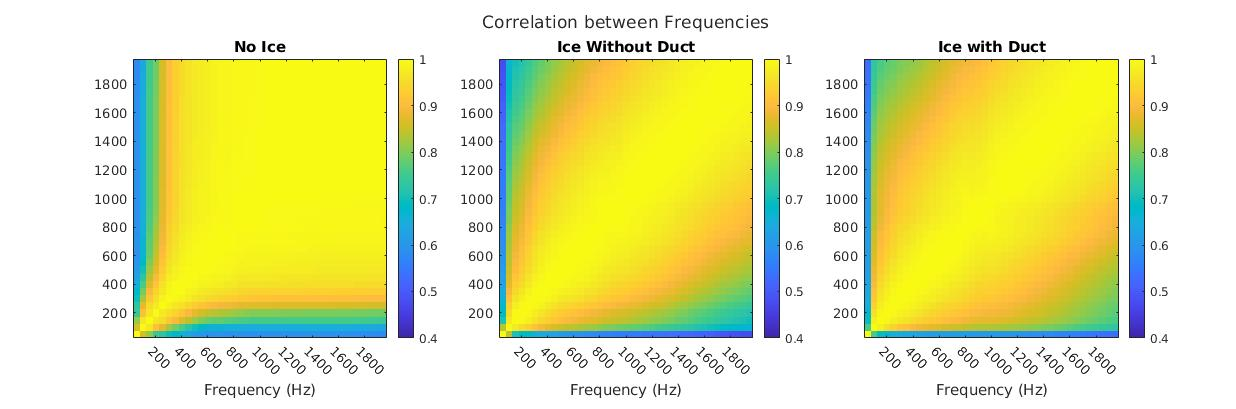
\includegraphics[scale=0.38]{Figures/corr_all_1x3.jpg}
\caption{Correlation between broadband frequencies for }
\label{fig_freq_corr}
\end{figure}

%%%%%%%%%%%%%%%%%%%%%%%%%%%%%%%%%%%%%%%%%%%%%%%%%%%%%%%%%%%%%%%%%%%%%%%%%%%%%%%%%%%%%%%%%%%%%
\subsection{The Ambient Noise Histogram} \label{sec_hist}
One of the simplest ways to visualize the differences between the three environmental conditions is by partitioning the ANL power spectral density (PSD) into histograms. After computing the sound pressure level (SPL) ANL, the bin size for each histogram was vector of 50 values, ranging from the minimum ANL to the maximum ANL of the frequency through all environmental conditions. The average bin size was around 1 Hz, with the highest frequencies having a slightly smaller bin size due to their more limited range. % julien note here?

Histograms were created using the probability density function (PDF) rather than counts to show the normalized likelihood of this ANL occurring. As the acoustic data is finite, an exact PDF is not possible, leading to an estimate function. The equation for this estimate is

\begin{equation} \label{eq:hist_pdf}
 \nu _{i}=\frac{c_{i}}{N \cdot w_{i}} 
\end{equation}

where $i$ refers to the bin, $\nu _{i}$ is the value of the bin, $c_{i}$ is the number of elements in the bin, and \textit{N} is the number of elements in the input data. The sum of all $\nu_{1}$, the bar size, is equivalent or almost equivalent to 1. Therefore, these histograms give the relative probability or makeup of a specific frequency's ANL in dB referenced to  $1 \mu Pa/Hz$ under the three acoustic environment conditions. From this, both the range of ambient noise and the most predominant levels are apparent. To demonstrate the conventions of an interpreting an ANL histogram, looking at a few significant figures showing the differences in acoustic environment levels is more pragmatic than examining 39 separate figures.

%%%%%%%%%%%%%%%%%%%%%%%%%%%%%%%%%%%%%%%%%%%%%%%%%%%%%%%%%%%%%%%%%%%%%%%%%
\subsubsection{Singular Frequency Histogram}
Figure \ref{fig_hist500} is an example of one histogram ranging from 450-550 Hz of the ANL for the three environmental conditions: 'ice with duct',  'ice without duct' and 'no ice'.  The blue histogram is 'ice with duct', the red histogram is 'ice without duct', and the yellow histogram is 'no ice.'  This coloring convention by acoustic environment holds for all statistic figures in this section. The number in the bins is less significant than the distribution of the histograms. 

Similar to the original paper's histogram centered at 300 Hz \footcite[]{Bonnel2021}, this example (\autoref{fig_hist500}) has three distinct peaks for each unique acoustic environment, displaying a key effect on underwater acoustics from changes to the Arctic environment.  It would appear that the quietest ambient levels occur under the 'ice without duct' condition with a highest occurring ANL of about 57 dB. The highest levels of ambient noise belongs to  the 'no ice' condition, with the most common level being around 80 dB. The levels for 'ice with duct' are between 'ice without duct' and 'no ice', with the most common level around 67 dB. 

In terms of shape, the 'no ice' condition histogram is the most normal or Gaussian in form and also has the shortest range from approximately 5-95 dB. 'Ice with duct' seems to have a normal shape, with some right skew and 'ice without duct' is skewed heavily to the right. The two ice conditions has similar ranges from about 62-95 dB, with a matching minimum dB value likely relating the mimimum dB detectable by the SHRUs at this frequency. This minimum detection threshold does change with frequency, as part of the initial setup of the DAQ. \footcite{daq process} %(note that this floor changes with Hz) 

It is commonly said that it is quieter under ice \footcite[]{ice_environ2}, and this figure directly reflects that through the distribution of sound levels in these three different bins. However, this histogram shows that the presence of the Beaufort duct \footcite[]{beaufortduct} increases the presence of louder ambient noise at this particular bandwidth of 500 Hz. When the duct is present, the ANL is likely to be 10 dB higher than an acoustic environment without the duct. Though the range of the two 'ice' conditions is similar,  their distributions are markedly different.  , but this strong difference is only present for a select range of frequencies. 


\begin{figure}[h]
\centering
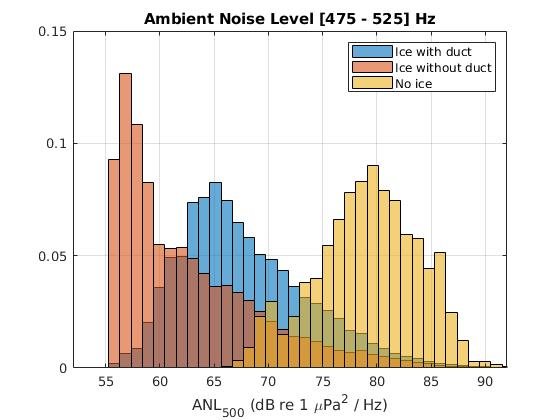
\includegraphics[scale=0.6]{Figures/ANL_500.jpg}
\caption{Histogram of normalized ANL at 500 Hz band for conditions Ice with duct (blue) }
\label{fig_hist500}
\end{figure}


%%%%%%%%%%%%%%%%%%%%%%%%%%%%%%%%%%%%%%%%%%%%%%%%%%%%%%%%%%%%%%%%%%%%%%%%%% order above?
\subsubsection{Multiple Frequencies of Ambient Noise Histograms Compared}
Interpreting one histogram allows its general attributes to be discussed, but more are needed to examine the intricacies of ANL over more frequencies.  For this section, four histograms at frequencies 250, 500, 1000, and 1500 Hz are presented on the same axes in \autoref{fig_selhist} for direct comparison, from 55 to 100 dB on the x-axis, and 0 to 0.25 on the y-axis. Both the distribution and shape of these ANL histograms changes as frequency increases. 

%\textbf{Distribution}

One of the most interesting aspects of the tri-colored \autoref{fig_hist500} is the sharp difference in layout between 'ice with duct' and 'ice without duct'. This phenomena of three separate peaks is only visible from approximately 100 to 700 Hz. The largest stratification between the three bins are between the frequencies of 150 Hz to 500 Hz. Beyond 700 Hz, the red and blue bars tend to overlap as the sound separation dissipates. This three peak ANL could be due to only a band of certain frequencies travelling well or noise in this band being generated into the Beaufort duct \footcite{beaufortduct} , though none of these reasons are certain.

The range of decibel levels covered by the three environmental conditions decreases as frequency increases. In the upper left of \autoref{fig_selhist}, the 250 Hz histogram for all three conditions has a range of almost 50 db, from approximately 57 to 100 dB. In contrast, the bottom right histograms at 1500 Hz cover a diminished range of 55 to 85 dB. The 35 dB long high frequency range is about 15 dB less than the low frequency range. The intermediate graphs of 500 and 100 Hz reflect this decreasing range of decibel values as the bar distribution becomes tighter.

In addition to the diminishing range, there is a general shift down in values for the three environmental conditions. The 'no ice' bars have peak makeup values at 85, 80, 77, and 75 for each increasing frequency. The maximum values of the bars also decrease with frequency for 'no ice', from above 0.1 to 0.75. 'No ice' is the loudest of the three conditions for all frequencies; its peak values are usually 10 to 20 dB more than the others. The other 'ice' environmental conditions do not behave similarly to the 'no ice' trends in ANL distribution.

The red bars for the 'ice without duct' histogram of \autoref{fig_selhist} shift down in peak value while increasing percentage as frequency goes up. At 250 Hz, the maximum bar value is just above 0.05 at 65 dB. When frequency increases for 'ice without duct' the minimum ANL value and maximum bar height tend to align, seen in the 500 Hz and 1000 Hz graphs. In the bottom right corner, the maximum bar height is almost 0.25 at 55 dB for 1500 Hz. 'Ice without duct' is always the minimum amount of ANL out of all three conditions through all frequencies.

The values for the blue bars of the 'ice with duct' histogram are usually somewhere between the values of 'no ice' and 'ice without duct'. 'Ice with duct' is similar to 'ice without duct' at the high frequencies, but differs in the mid to low bands. At 250 and 500 Hz the peak values for 'ice with duct' are between those of 'no ice' and 'ice without duct'. 250 Hz has a 10 dB difference (65-75-85) between each condition, but 500 Hz has a smaller gap between 'ice' conditions (57 to 65 dB) and 'no ice' (65 to 80 db). The red and blue bars align at 1000 and 1500 Hz as the minimum ANL becomes the most predominant noise level. The most predominant value, though not the minimum ANL is around 57 dB. As frequency increases, the maximum bar height also increase, from 0.1 to 0.15, which is less than the 'ice without duct' bar height increase.

\begin{figure}[h]
\centering
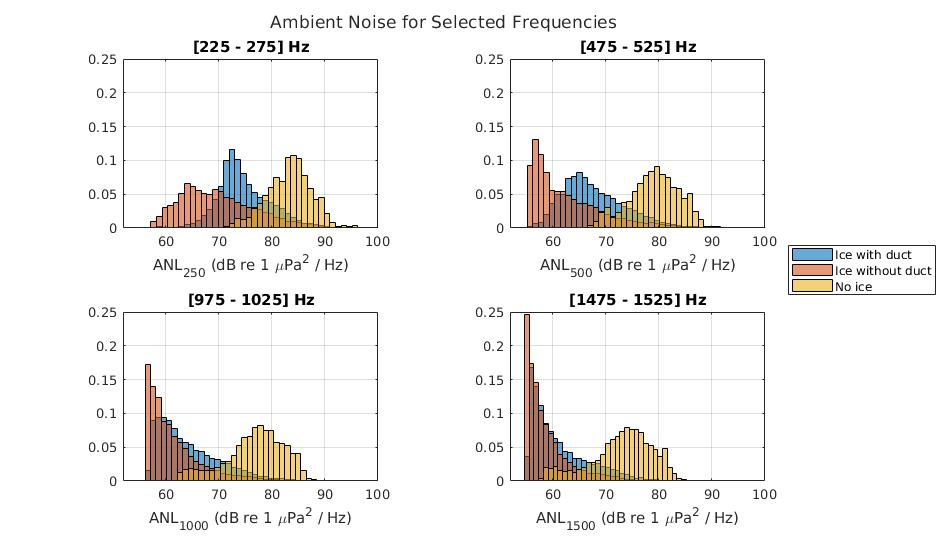
\includegraphics[scale=0.45]{Figures/selected_hists.jpg}
\caption{Histograms of ANL for 250, 500, 1000, and 1500 Hz}
\label{fig_selhist}
\end{figure}
%\textbf{Shape}

The shape of the histograms varies highly throughout the frequencies examined. For 250 Hz and below all three environmental conditions have a fairly normal shape, but above 250 Hz the shapes diverge for all three. The 'no ice' histogram maintains a mostly normal shape through the whole range of frequencies. Without ice to dampen it, ambient sound is likely wind and ocean driven. Toward the highest frequencies, there is a bit of left skew to the 'no ice' histograms, which may be related to the lowered presence of the high frequencies altogether. It does not follow the pattern of the ice environmental condition histograms.

Most of the changes in shape are seen in the red and blue histograms of the ice environment. Above 250 Hz, the 'ice without duct' histogram becomes predominantly right skewed. This right skew for 'ice without duct' emphasizes that the highest occurring noise levels are the lowest values, and that the minimum sound levels occur under 'ice without duct'.  'Ice with duct' is normal in shape from 50 to about 350 Hz, above 500 Hz is begins to be skewed right. At around 900 Hz, the histograms for 'ice with duct' and 'ice without duct' are both right skewed and have heavy overlap. The right skew and overall shift down in values reflect the quieter nature of sound under ice and at higher frequency. It is apparent that there is more sound with ice than without.

% what does it mean



%%%%%%%%%%%%%%%%%%%%%%%%%%%%%%%%%%%%%%%%%%%%%%%%%%%%%%%%%%%%%%%%%%%%%%%%%
\subsection{Average ANL} \label{sec_avg_anl}
Several single numeral metrics for describing the overall behavior of ANL in frequency present trends that cannot be seen through examining histogram graphs alone. \autoref{fig_avg_anl} shows the average ambient noise level of each environmental condition for frequencies 50 to 1900. This average value is taken across the whole yearlong time frame of acoustic data being recorded.  ANL is in dB referenced to $ 1 \mu Pa^{2}/Hz$ are the units of the y-axis and frequency is on the x-axis. The averages for 'ice with duct' are in blue, the averages for 'ice without duct' are in red, and the 'no ice' is in yellow.

A caveat for using the average value as a descriptor is the tendencies to of the data to be skewed, as seen in \autoref{fig_selhist}. A general negative trend in average ANL is present across all three acoustic environment types. 'No ice' behaves linearly while the 'ice' conditions behave more exponentially. Both 'ice' conditions begin to slow the descent of ANL around 600 Hz. There are small increases every four points or so in the data, perhaps caused by the n-50 band being slightly more active at that point. The three lines of \autoref{fig_avg_anl} definitively show that 'no ice' is the loudest of the three conditions for the majority of the frequencies, followed by 'ice with duct'. The lowest levels of ANL typically reside in 'ice without duct'.

When there is no ice, ambient noise can come from a variety of sources including rain, waves, and wind. In addition, shipping in the general area can create a significant quantity of propeller noise as decreased ice leads to higher volume of ship traffic. \footcite[]{ship_traffic} When there is ice, most of the ambient noise in the Arctic when there is ice is generated by the movement of the ice itself - grinding, slipping, and shearing. It would seem the presence of the Beaufort duct increases the average ANL for many frequencies above the normal condition of 'ice without duct'. 
%Things to consider: what else functions in these bandwidths of activity, like whales and other biologic factors? Is what we do going to negatively impact them?



\begin{figure}[p]
\centering
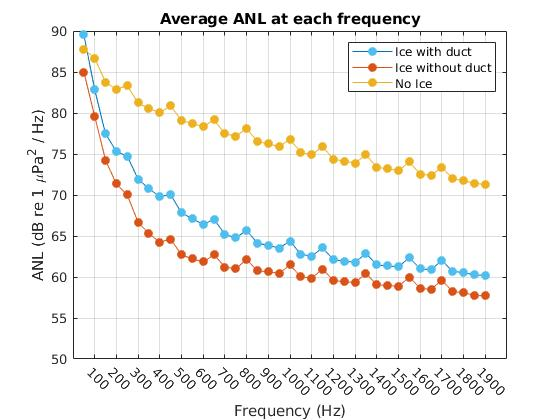
\includegraphics[scale=0.6]{Figures/Average_ANL.jpg}
\caption{Average ANL at frequencies from 50 to 1900 Hz.}
\label{fig_avg_anl}
\end{figure}

% mode cutoof is at 1950, change and LoCK axis corrds to match
\begin{figure}[p]
\centering
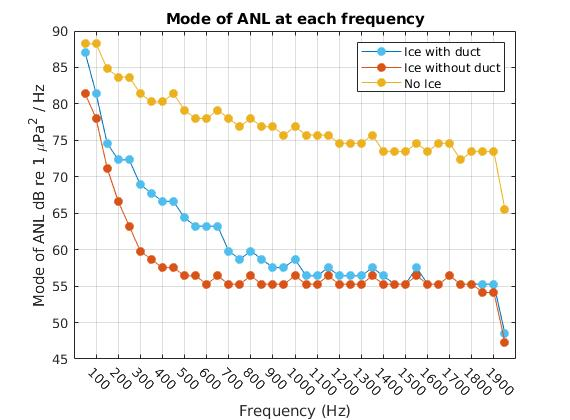
\includegraphics[scale=0.6]{Figures/mode_ANL_allfreqs.jpg}
\caption{Mode or highest occuring bin value of ANL for frequencies from 50 to 1900 Hz.}
\label{fig_mode}
\end{figure}

%%%%%%%%%%%%%%%%%%%%%%%%%%%%%%%%%%%%%%%%%%%%%%%%%%%%%%%%%%%%%%%%%%%%%55
\subsection{ANL Approximate Modes}

Another single metric for describing the general nature of ANL under an environmental condition at each frequency is the approximate mode of the data. While an exact mode was not possible for noise levels with multiple decimal places, an estimate was made using the highest bars of the bin edges in \autoref{sec_hist}. As opposed to the average, this statistic metric leans heavily into the skew of the histogram. Looking at the mode may be better for describing the general trends of each acoustic environment's frequency. When compared, \autoref{fig_avg_anl} and \autoref{fig_mode} display different changes in ANL and frequency. 

% what is going on in mode
The yellow points denoting the modes for 'no ice' have the loudest modes, beginning at almost 90 dB and tapering down to approximately 75 dB. The curve of the 'no ice' line is nowhere near as steep as the ANL modes for 'ice with duct' and 'ice without duct'. The blue points representing the modes of 'ice with duct' begin around 87 dB, close to 'no ice'. A steep drop in decibel mode occurs from 100 Hz to 700 Hz, where the modes begin to plateau around 57 dB.  The red points for the modes of 'ice without duct' behave similarly to 'ice with duct', but the decrease in ANL is more significant at a lower frequency. 'Ice without duct' begins its mode plateau of 55 dB at 500 Hz.

For the lowest frequencies within \autoref{fig_mode}, the different between ANL is less than 10 dB, though by 200 Hz this difference has increased to almost 20 dB. From 50 to 1000 Hz, the modes for 'ice with duct' remain between those of 'no ice' and 'ice without duct'. After this, overlap between the ice conditions occurs. Similar to previous sections, 'no ice' is typically the loudest environmental condition, followed by 'ice with duct', then 'ice without duct'. \autoref{fig_mode} does offer some key differences to this generalized pattern of sound level.

Unlike \autoref{fig_mode}, it appears that 'ice with duct' and 'ice without duct' share their most predominant ANL of 55 Hz. The stratification in their averages is lost when modes are compared, suggesting that at frequencies above 500 Hz, the Beaufort duct is not as prevalent a factor. The mode line for 'no ice' is less steep than the average line for 'no ice', though the two run in generally the same ranges. 

Modes are statistically the highest occurring sound level recorded by the SHRUs, and are therefore the most likely to occur under the environmental conditions presented in the future. In general, all the mode values for each frequency in \autoref{fig_mode} are lower than those of the average values in \autoref{fig_avg_anl}. Comparing these modes numerically could show potential overall ambient noise level changes to the Arctic underwater noise environment.  


%%%%%%%%%%%%%%%%%%%%%%%%%%%%%%%%%%%%%%%%%%%%%%%%%%%%%%%%%%%%%%%%%%%%%%%%%%%%%%%%
\subsection{Pairwise Difference} \label{sec_pairdiff}

Using modes to generalize the ANL for each frequency above 1000 Hz, the ANL for 'ice with duct' and 'ice without duct' are almost the same. Comparing the differences between these modes is a reasonable method for finding a significant metric of the change between conditions. The metric used to make such a comparison is the pairwise difference between these probability distributions. Pairwise difference is the length between two bins at the same frequency between the two environmental noise types being analyzed. 

This metric is not measure of probability but is the difference between the highest probable ANL of each acoustic condition. Pairwise difference in the context of this analysis means the difference between each environmental condition's noise level of the highest histogram bar of the probability distribution, not the highest level of noise recorded. Because the data being compared is a decibel value, the resulting parameter is in terms of noise, and is not a probability. The pairwise difference for this analysis was calculated using the following equation:

%pair_dist_duct_noduct(i)=edges_duct(ind_duct(i))-edges_no_duct(ind_no_duct(i))
\begin{equation}
PD(\mathcal{A},\mathcal{B},\omega)=\mid argmax(\mathcal{H}_{i} [ANL ^{A}(\omega))]-argmax(\mathcal{H}_{i} [ANL^{B}\omega)]\ \mid 	% this is not actual stat distance 
\end{equation}
% argmax of hist-argmaxofhist, repeat equation

Where $\mathcal{H}_{i}$ refers to the histogram bin, $ANL^{\mathcal{A/B}}$ is the ambient noise at an environmental condition, $\omega$ is the frequency of interest, and $\mathcal{A/B}$ refer to the two acoustic environments being compared. As discussed above, $PD$ is not a value of probability, but a decibel measure of the difference between environments. It directly compares two decibel values between two environmental conditons. The x-axis of this graph is frequency in Hz, while the y-axis is the difference in ANL in dB. The three environmental conditions produce three environmental coupling differences, marked by three new point and line colors. \autoref{fig_pairwisedist} labels the environments being compared through pairwise distance with a color combination of environments that are the secondary mixes of the primary colors of \autoref{fig_avg_anl}. Purple is the difference between 'ice with duct' and 'ice without duct', green is the difference between 'ice with duct' and 'no ice', and orange is the difference between 'ice without duct' and 'no ice'


The conditions with the highest overall difference are 'no ice' and 'ice without duct' which are represented by the orange points. This orange line could represent the typical difference between the ambient noise with and without ice prior to the introduction of the Beaufort duct. It begins with a steep increase in dB from 50 Hz to 500 Hz, reaching a top difference of 24 dB at 450 Hz. After, the difference between 'ice without duct' and 'no ice' begins to decrease slightly, hovering around a 20 dB difference from 500 to 1900 Hz.

The middle difference condition comparison is between 'ice with duct' and 'no ice', represented by a green line and points. Beginning with a pairwise difference of 1 dB at 50 Hz, this line also climbs, though not as quickly as the orange line. The difference between 'ice with duct' and 'no ice' reaches a maximum of 19 dB at 900 Hz and settles around 18 dB until 1900. Above 1000 Hz, the pairwise difference for the orange and green lines are very similar, suggesting that there isn't a strong difference between the 'ice with duct' and 'ice without duct' noise levels when compared with 'no ice'. This  similarity between 'ice' conditions is emphasised by the third pairwise difference line.

The third pairwise difference is the conditions with the lowest overall difference of 'ice with duct' and 'ice without duct', represented by purple points. Starting with a 6 dB difference at 50 Hz, there is a small decrease before the pairwise difference between 'ice with duct' and 'ice without duct' maxes out at 9 dB. Following this maxima, the decibel values steadily decline before going near zero from 1100 Hz on. For half of its points, the purple line is more than 15 dB below the other two line's differences.  

This graph shows that the conditions 'ice with duct' and 'ice no duct' are very similar, while the conditions 'ice no duct' and 'no ice' are most different in ANL. One of the most interesting aspects of \autoref{fig_pairwisedist} is the insight into the significant band of frequencies the Beaufort duct seems to affect the most. From 200 Hz to 600 Hz, the highest pairwise difference between these conditions occurs at an average of 8 dB. This significant band is again reflected in the most separation between the orange and green lines occurring from 200 Hz to 600 Hz. The ambient noise of an environment with the duct is higher in ANL than an environment without the duct, resulting in smaller differences when compared to an ice-free environment. However, the stratification between 'ice with duct' and 'ice without duct' does not encompass all frequencies, demonstrated by the overlap between the orange and green lines as frequency increases.

%%%%%%%%%%%%%%%%%%%%%%%%%%%%%%%%%%%%%%%%%%%%%%%%%%%%%%%%%%%%%%%%%%%%%%%%%%%%%%
% figures of total vart dist and pairwise dist
\begin{figure}[p]
\centering
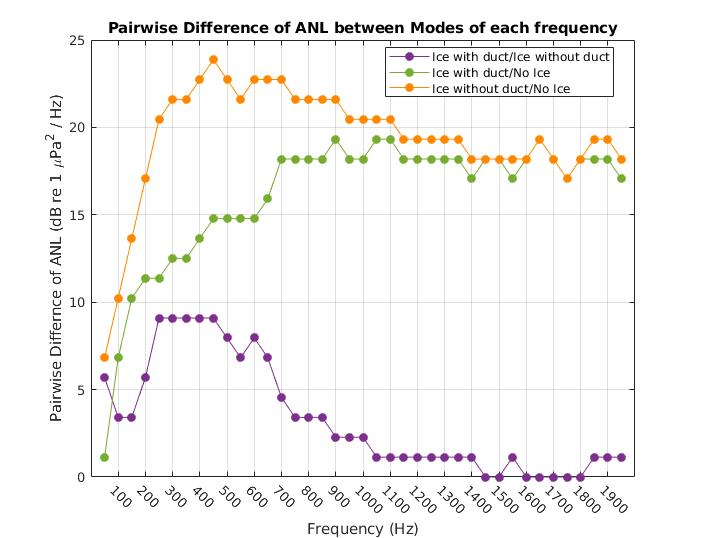
\includegraphics[scale=0.6]{Figures/recolor_pairwise_dist_ANLs.jpg}
\caption{Pairwise distance for frequencies from 50 to 1900 Hz.}
\label{fig_pairwisedist}
\end{figure}

%% FIX LEGEND AGAIN
\begin{figure}[p]
\centering
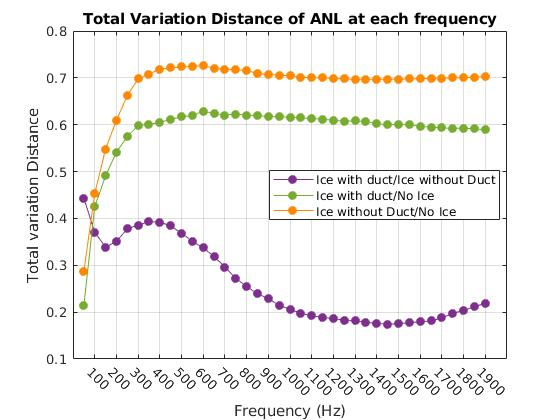
\includegraphics[scale=0.62]{Figures/recolor_total_var_dist_norm_pdf.jpg}
\caption{Total Variation distance for frequencies from 50 to 1900 Hz.}
\label{fig_totvardist}
\end{figure}

%%%%%%%%%%%%%%%%%%%%%%%%%%%%%%%%%%%%%%%%%%%%%%%%%%%%%%%%%%%%%%%%%%%%%%%%%%%%%%%%%%%
\subsection{Total Variation Distance} \label{sec_tvd}
Rather than examine the statistic quantities of each acoustic environmental condition alone, one can compare the relationship between environments by frequency through total variation distance (TVD). This metric shows the likelihood between two probability distributions of acoustic environments. Unlike \autoref{sec_pairdiff}, this metric is a normalized value of probability, not a measure of sound level in decibels. Total variation distance essentially is the absolute area between two curves, showing how likely acoustic conditions will have overlap in their ANL distributions. 

 Total variation distance looks at all the data across all the frequencies, with the count of each bin as a proportion. It takes every value of the probability of that bin and takes the sum of the absolute difference between the two. TDV is not a measure of ANL in dB but a measure of probability of occurrence between two conditions. This data set was normalized using PDF similar to the histograms in \autoref{sec_hist}. For the purposes of this analysis, the total variation distance uses the following equation: 

% equation used for our analysis
%\begin{equation} \label{eq:actualtotvar}
%\delta(Duct, No Duct)=\frac{1}{2} \Sigma \mid Duct(f) - No Duct(f) \mid 
%\end{equation}

\begin{equation} \label{tdv_eq}
    \delta ^{TVD} _{ANL} ( \mathcal{A}, \mathcal{B}, \omega) = \frac{1}{2} \sum _{i} ^{} \mid \mathcal{H}_{i} [ANL^{\mathcal{A}}(\omega)] -\mathcal{H}_{i} [ANL^{\mathcal{B}}(\omega)] \mid 
\end{equation}

where  $\mathcal{H}_{i}$ is the \textit{i}th bin of the environmental condition histogram $\cal{H}$, $\omega$ is the frequency band, and $\cal{A/B}$ refer to the different environmental condition being compared. $\delta$ is the total variation difference between two ANL histograms of different environmental conditions. One number is returned by this equation that sums up the total variation distance between the two conditions. A value of 1 means that two probability distributions are entirely different with no shared ANL values. An output value of 0 means the probability distribution are exactly the same, with the same occurrence of each ANL value.

\autoref{fig_totvardist} uses the same coloring convention as \autoref{fig_pairwisedist}, where purple is the difference between 'ice with duct' and 'ice without duct', green is the difference between 'ice with duct' and 'no ice', and orange is the difference between 'ice without duct' and 'no ice'. The x-axis are TVD values ranging from 0.1 to 0.8. This single metric defining the relationship between two environmental conditions is plotted against frequency fgrom 50 Hz to 1900 Hz, keeping with the rest of the statistic figures.

 The highest variation distance between the conditions ‘ice with duct' and 'ice without duct’ occurs at 50 Hz at a value of 0.44. The highest variation distance between 'ice with duct' and 'No Ice' occurs at 600 Hz with a distance of 0.63. The highest variation distance for 'no ice' and 'ice without duct' occurs at 600 Hz and at a value of 0.72. At no point do the probability distributions for the three environmental conditions not overlap in ANL, though what dB values relate the two are not known. 

The highest TVD line is the relationship between 'no ice' and 'no duct', represented by the orange points. Beginning at 0.3, the line increases from 50 Hz to 400 Hz and then plateaus at a value of 0.7. This indicates that the probability distributions for 'ice without duct' and 'no ice' do not have much in common and are quite different. Looking at \autoref{fig_selhist} validates this, as the red and yellow bars of the respective histograms vary highly in shape.

The middle green line represents the TVD between the environmental conditions of 'ice with duct' and 'no ice'. Similar to the orange line, The green points rapidly increase from 50 Hz to 600 Hz, before declining and plateauing around 0.6 for the higher frequencies. This indicates that the probability distributions for 'ice with duct' and 'no ice' do have some overlap, but are still more than 50\% different from each other. They are not as different as the conditions 'ice without duct' and 'no ice'. 

The lowest TVD values belong to the conditions 'ice with duct' and 'ice without duct', showing that these two conditions are the most similar. The purple line begins below a value of 0.5, which is also the highest value achieved by the purple line. The TVD decrease to 0.35, before a slight increase from 150 Hz to 300 Hz to a TVD of 0.4. Then the points decline under a TVD of 0.2 until 1200 Hz, where there is another slight increase to above 0.2. From 800 to 1900 Hz, it can be assumed that there is a significant amount of similarity in probability distributions between 'ice with duct' and 'ice without duct'. 

Similar to \autoref{fig_pairwisedist}, total variation distance shows that there is a significant band of frequencies where the difference between ambient noise with and without the Beaufort duct is amplified. From 100 to 800 Hz, the purple line representing the difference between ice with duct and ice without duct is higher than the rest of the points. This is also corroborated by the green and orange line increasing in TVD through a similar band of frequency. When the TVD vales for 'ice with duct' and 'ice without duct' are highest, the TVD values for the green and orange points are lowest. Additionally, total variation distance as a whole is lower when the duct is present when compared to an ice-free environment. This suggests that the sound makeup under these two environments is more similar than a traditionally duct-free area, likely attributed to ambient noise with the duct being closer to an ice free Arctic.

%%%%%%%%%%%%%%%%%%%%%%%%%%%%%%%%%%%%%%%%%%%%%%%%%%%%%%%%%%%%%%%%%%%%%%%%%%%
% ADDITIONAL POSSIBLE SECTIONS?
% MAX, min, difference maxmin
% more histograms


%%%%%%%%%%%%%%%%%%%%%%%%%%%%%%%%%%%%%%%%%%%%%%%%%%%%%%%%%%%%%%%%%%%%%%%%%%%%%%
% can always add more like max min covariance more histograms, etc

% the end of statistic section
\section{Probability and Statistics Conclusions}
% a summary of the results from above 'the what it means' section
Using different probability and statistics, certain generalizations about the soundscape of ambient noise in the Arctic can be made. Expanding the frequency of interest from 300 Hz to a significantly wider bandwidth of 1850 Hz increases the understanding of how ambient noise operates in the Arctic sea. The probability distributions of ambient noise show a 45 dB range of sound received between all three environmental conditions. As frequency increases, ANL is likely to decrease, with a minimum ambient noise around 55 dB. A clear difference between louder sound without ice and quieter sound with ice, regardless of duct, exists as well. This decibel difference changes highly with frequency, something not seen before.

From this section, it is apparent that the Beaufort duct has a strong effect on the level of noise under ice in the Arctic. The probability of the duct's presence raising the ambient noise by almost 10 dB is high when compared to a ductless environment. However, this increase in noise is limited to a certain band of frequencies of about 100 to 700 Hz. It is unlikely that the duct would cause the same ANL increase at higher frequencies. This results in similar noise levels above 100 Hz, regardless of whether the duct is present or not.

